\uuid{2ynq}
\exo7id{7697}
\auteur{mourougane}
\organisation{exo7}
\datecreate{2021-08-11}
\isIndication{false}
\isCorrection{true}
\chapitre{Sous-variété}
\sousChapitre{Sous-variété}

\contenu{
\texte{

}
\begin{enumerate}
    \item \question{La courbe paramétrée suivante est-elle régulière ?
$$\begin{array}{ccc}
 c: \Rr &\to&\Rr ^3\\ t&\mapsto& \left(\begin{array}{c}t\cos t \\ t\sin t\\ t\end{array}\right).
\end{array}$$}
\reponse{Les composantes de l'application $c$ sont de classe $\mathcal{C}^\infty$.
 La dérivée de la dernière composante n'est jamais nulle.
 La courbe $c$ est donc régulière.}
    \item \question{On fixe deux nombres réels $a<b$. Comparer la longueur de la portion de la courbe $c$ 
paramétrée par $[a,b]$ et $\sqrt{2}(b-a)$.}
\reponse{Pour tout paramètre $t$, $\|\dot{c}(t)\|=\sqrt{2+t^2}\geq \sqrt{2}$.
 Donc,
 $$L[c_{\mid [a,b]}]=\int_a^b \|\dot{c}(t)\| dt\geq\sqrt{2}(b-a).$$}
    \item \question{Déterminer une surface quadrique qui contient l'image $\mathcal{C}$ de la courbe $c$.}
\reponse{Soit $t\in\Rr $,
 $$(t\cos t)^2+(t\sin t)^2=t^2=(t)^2.$$
 Par conséquent, $\mathcal{C}$ est dans la quadrique d'équation $x^2+y^2=z^2$.}
    \item \question{Déterminer un déplacement (non égal à l'identité) de l'espace $\Rr ^3$ qui conserve l'image $\mathcal{C}$ de la courbe $c$.}
\reponse{Soit $t\in\Rr $, $c(-t)= \left(\begin{array}{c}-t\cos t \\ t\sin t\\- t\end{array}\right)$ et se déduit donc de $c(t)$
 par le demi-tour autour de l'axe des ordonnées (d'équation $x=z=0$).}
    \item \question{Décrire l'allure de la courbe $\mathcal{C}$.}
\reponse{$$ 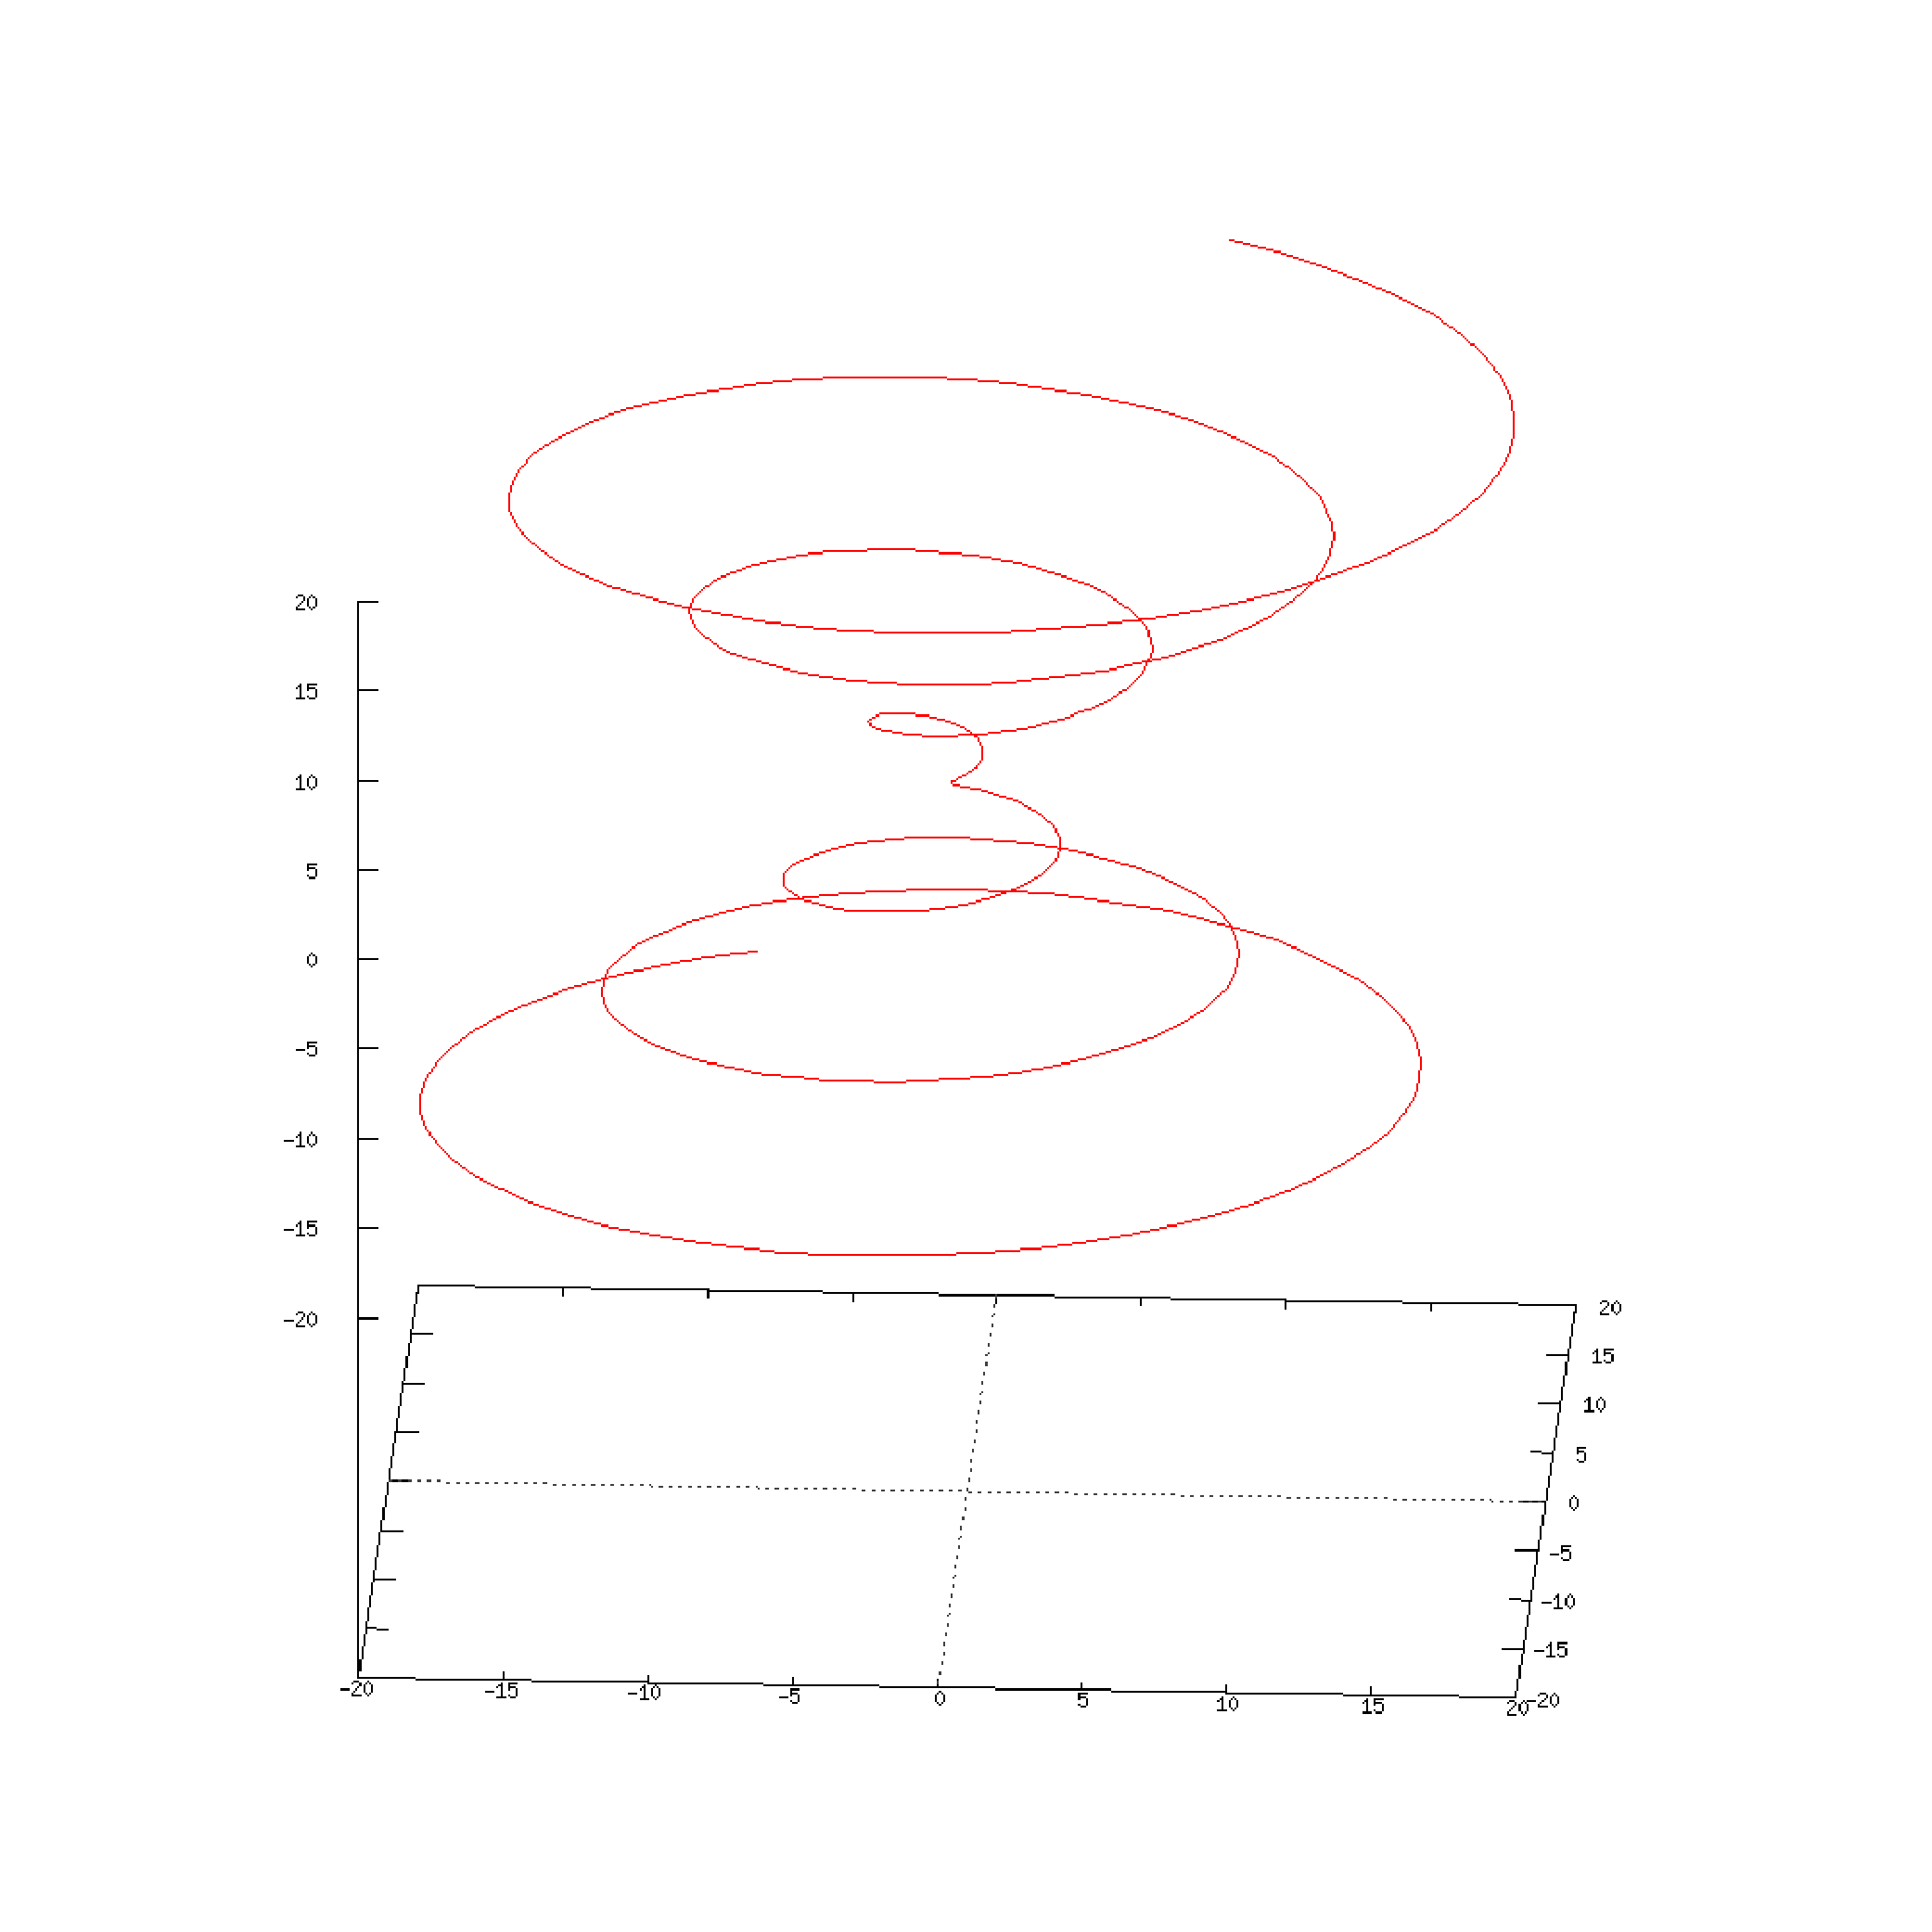
\includegraphics[scale=.4]{images/img-mour-449}$$
 %faire du gif avec wims2
 %convert wims.gif wims.png}
    \item \question{Calculer la fonction torsion de la courbe $c$.}
\reponse{$$c(t)=\left(\begin{array}{c}t\cos t \\ t\sin t\\ t\end{array}\right) ; 
 \dot{c}(t)=\left(\begin{array}{c}\cos t -t\sin t\\ \sin t + t\cos t\\ 1\end{array}\right) ;$$
 $$
 \ddot{c}(t)=\left(\begin{array}{c}-2\sin t -t\cos t\\ 2\cos t - t\sin t\\ 0\end{array}\right) ; 
 \dddot{c}(t)=\left(\begin{array}{c}-3\cos t +t\sin t\\ -3\sin t -t\cos t\\ 0\end{array}\right).$$
 Ainsi, $$\det\begin{pmatrix}
        \cos t -t\sin t &-2\sin t -t\cos t&-3\cos t +t\sin t\\
 \sin t + t\cos t&2\cos t - t\sin t&-3\sin t - t\cos t\\1&0&0
        \end{pmatrix}=t^2+6$$
 Par ailleurs,
 $$\dot{c}(t)\wedge\ddot{c}(t)=\left(\begin{array}{c}\cos t -t\sin t\\ \sin t + t\cos t\\ 1\end{array}\right) 
 \wedge\left(\begin{array}{c}-2\sin t -t\cos t\\ 2\cos t - t\sin t\\ 0\end{array}\right)=
 \begin{pmatrix}
 - 2\cos t +t\sin t\\-2\sin t -t\cos t\\2+t^2
 \end{pmatrix}
 $$ dont la norme au carré est $t^4+5t^2+8$.
 La fonction torsion de $c$ est donc $$\tau(t)=\frac{t^2+6}{t^4+5t^2+8}.$$}
\end{enumerate}
}
